%% abtex2-modelo-relatorio-tecnico.tex, v-1.9.7 laurocesar
%% Copyright 2012-2018 by abnTeX2 group at http://www.abntex.net.br/ 
%%
%% This work may be distributed and/or modified under the
%% conditions of the LaTeX Project Public License, either version 1.3
%% of this license or (at your option) any later version.
%% The latest version of this license is in
%%   http://www.latex-project.org/lppl.txt
%% and version 1.3 or later is part of all distributions of LaTeX
%% version 2005/12/01 or later.
%%
%% This work has the LPPL maintenance status `maintained'.
%% 
%% The Current Maintainer of this work is the abnTeX2 team, led
%% by Lauro César Araujo. Further information are available on 
%% http://www.abntex.net.br/
%%
%% This work consists of the files abntex2-modelo-relatorio-tecnico.tex,
%% abntex2-modelo-include-comandos and abntex2-modelo-references.bib
%%

% ------------------------------------------------------------------------
% ------------------------------------------------------------------------
% abnTeX2: Modelo de Relatório Técnico/Acadêmico em conformidade com 
% ABNT NBR 10719:2015 Informação e documentação - Relatório técnico e/ou
% científico - Apresentação
% ------------------------------------------------------------------------ 
% ------------------------------------------------------------------------

\documentclass[
	% -- opções da classe memoir --
	12pt,				% tamanho da fonte
	openright,			% capítulos começam em pág ímpar (insere página vazia caso preciso)
	twoside,			% para impressão em recto e verso. Oposto a oneside
	a4paper,			% tamanho do papel. 
	% -- opções da classe abntex2 --
	%chapter=TITLE,		% títulos de capítulos convertidos em letras maiúsculas
	%section=TITLE,		% títulos de seções convertidos em letras maiúsculas
	%subsection=TITLE,	% títulos de subseções convertidos em letras maiúsculas
	%subsubsection=TITLE,% títulos de subsubseções convertidos em letras maiúsculas
	% -- opções do pacote babel --
	english,			% idioma adicional para hifenização
	french,				% idioma adicional para hifenização
	spanish,			% idioma adicional para hifenização
	brazil,				% o último idioma é o principal do documento
	]{abntex2}


% ---
% PACOTES
% ---

% ---
% Pacotes fundamentais 
% ---
\usepackage{lmodern}			% Usa a fonte Latin Modern
\usepackage[T1]{fontenc}		% Selecao de codigos de fonte.
\usepackage[utf8]{inputenc}		% Codificacao do documento (conversão automática dos acentos)
\usepackage{indentfirst}		% Indenta o primeiro parágrafo de cada seção.
\usepackage{color}				% Controle das cores
\usepackage{graphicx}			% Inclusão de gráficos
\usepackage{microtype} 			% para melhorias de justificação
\usepackage{amsmath}
\usepackage{amsfonts}
\usepackage{float}
% ---

% ---
% Pacotes adicionais, usados no anexo do modelo de folha de identificação
% ---
\usepackage{multicol}
\usepackage{multirow}
% ---
	
% ---
% Pacotes adicionais, usados apenas no âmbito do Modelo Canônico do abnteX2
% ---
\usepackage{lipsum}				% para geração de dummy text
% ---

% ---
% Pacotes de citações
% ---
\usepackage[brazilian,hyperpageref]{backref}	 % Paginas com as citações na bibl
\usepackage[alf]{abntex2cite}	% Citações padrão ABNT


% ---
%MINHAS PERSONALIZAÇÕES
% ---
\usepackage{rotating}
\usepackage{booktabs} % Para melhor formatação de tabelas
\usepackage{caption}  % Para customização das legendas
\usepackage[margin=1in]{geometry}
\usepackage{titlesec}


% Redefine o comando de capítulo para não começar em uma nova página
\titleformat{\chapter}[block]
  {\normalfont\huge\bfseries}{\ \ \thechapter}{20pt}{\Huge}
\titlespacing*{\chapter} 
{0pt}{1pt}{1pt}
\titlespacing*{\section}
  {0pt}{1pt}{1pt}
\titlespacing*{\subsection}
  {0pt}{1pt}{1pt}
\titleclass{\chapter}{straight}

\setlength{\intextsep}{10pt}

\setlist[itemize]{noitemsep, topsep=0pt}
\setlength{\abovedisplayskip}{1pt} % espaçamento acima das equações
\setlength{\belowdisplayskip}{1pt} % espaçamento abaixo das equações
\setlength{\abovedisplayshortskip}{1pt} % espaçamento curto acima das equações
\setlength{\belowdisplayshortskip}{1pt} % espaçamento curto abaixo das equações

% Ajuste do espaçamento ao redor do ambiente aligned
\setlength{\abovedisplayshortskip}{1pt}
\setlength{\belowdisplayshortskip}{1pt}


% --- 
% CONFIGURAÇÕES DE PACOTES
% --- 

% ---
% Configurações do pacote backref
% Usado sem a opção hyperpageref de backref
\renewcommand{\backrefpagesname}{Citado na(s) página(s):~}
% Texto padrão antes do número das páginas
\renewcommand{\backref}{}
% Define os textos da citação
\renewcommand*{\backrefalt}[4]{
	\ifcase #1 %
		Nenhuma citação no texto.%
	\or
		Citado na página #2.%
	\else
		Citado #1 vezes nas páginas #2.%
	\fi}%
% ---

% ---
% Informações de dados para CAPA e FOLHA DE ROSTO
% ---
\titulo{Relatório da 5ª prática}
\autor{Romário Jonas de Oliveira Veloso}
\local{Recife - PE}
\data{2024}
\instituicao{%
  Universidade Federal de Pernambuco (UFPE)
  \par
  Centro de Tecnologia e Geociências (CTG)
  \par
  Departamento de Eletrônica e Sistemas (DES)}
\tipotrabalho{Relatório técnico}
% O preambulo deve conter o tipo do trabalho, o objetivo, 
% o nome da instituição e a área de concentração 
\preambulo{Relatório Técnico para a disciplina Circuitos Elétricos 2, período 2024.1.}
% ---

% ---
% Configurações de aparência do PDF final

% alterando o aspecto da cor azul
\definecolor{blue}{RGB}{41,5,195}

% informações do PDF
\makeatletter
\hypersetup{
     	%pagebackref=true,
		pdftitle={\@title}, 
		pdfauthor={\@author},
    	pdfsubject={\imprimirpreambulo},
	    pdfcreator={LaTeX with abnTeX2},
		pdfkeywords={abnt}{latex}{abntex}{abntex2}{relatório técnico}, 
		colorlinks=true,       		% false: boxed links; true: colored links
    	linkcolor=blue,          	% color of internal links
    	citecolor=blue,        		% color of links to bibliography
    	filecolor=magenta,      		% color of file links
		urlcolor=blue,
		bookmarksdepth=4
}
\makeatother
% --- 

% --- 
% Espaçamentos entre linhas e parágrafos 
% --- 

% O tamanho do parágrafo é dado por:
\setlength{\parindent}{1.3cm}

% Controle do espaçamento entre um parágrafo e outro:
\setlength{\parskip}{0.2cm}  % tente também \onelineskip

% ---
% compila o indice
% ---
\makeindex
% ---

% ----
% Início do documento
% ----
\begin{document}

% Seleciona o idioma do documento (conforme pacotes do babel)
%\selectlanguage{english}
\selectlanguage{brazil}

% Retira espaço extra obsoleto entre as frases.
\frenchspacing 

% ----------------------------------------------------------
% ELEMENTOS PRÉ-TEXTUAIS
% ----------------------------------------------------------
% \pretextual

% ---
% Capa
% ---
\imprimircapa
% ---

% ---
% Folha de rosto
% (o * indica que haverá a ficha bibliográfica)
% ---
\imprimirfolhaderosto*
% ---


% ---
% inserir o sumario
% ---
%\pdfbookmark[0]{\contentsname}{toc}
%\tableofcontents*
%\cleardoublepage
% ---


% ----------------------------------------------------------
% ELEMENTOS TEXTUAIS
% ----------------------------------------------------------
\textual



\chapter{Introdução}
Neste laboratório, projetaremos e testaremos um filtro ativo passa-alta Butterworth de 4ª ordem, analisando e medindo o comportamento da magnitude de sua resposta em frequência.
Esta prática está dividida em duas partes. A primeira parte é o projeto e a análise teórica do circuito em questão. Na segunda parte, faremos a montagem física do circuito em protoboard e mediremos a tensão de saída para verificarmos os resultados teóricos.


\chapter{Objetivos Gerais}
Projetar um filtro-protótipo ativo passa-alta Butterworth, aplicar escalonamento de frequência e magnitude, usar transformada de Laplace, medir grandezas elétricas com osciloscópio, comparar comportamento na frequência dos filtros e resolver equações algébricas com SymPy.


\chapter{Objetivos Específicos}
\begin{itemize}
    \item Determinar a função de transferência do filtro-protótipo.
    \item Calcular os valores dos elementos do circuito para a implementação do filtro.
    \item Ajustar os valores dos elementos do circuito para os valores comerciais mais próximos.
    \item Comparar o comportamento na frequência do filtro projetado com o comportamento teórico esperado.
    \item Utilizar ferramentas de simulação computacional, como LTSpice, para validar os resultados teóricos.
    \item Realizar medições práticas em laboratório para verificar o comportamento do filtro projetado.
\end{itemize}


\clearpage
\chapter{Metodologia}

\section{Equipamentos e Materiais Necessários}
Para a realização desta prática, serão utilizados tanto softwares específicos quanto componentes eletrônicos. Os recursos computacionais incluem:
\begin{itemize}
    \item Jupyter Notebook;
    \item LTSpice;
    \item Osciloscópio \cite{keysight_manual};
    \item Fonte de tensão;
    \item Multímetro \cite{keysight-u1250};
    \item Resistores e capacitores de acordo com o projeto;
    \item Amplificador operacional LM324 \cite{lm324_datasheet}.
\end{itemize}

Com os materiais e softwares preparados, o próximo passo envolve a análise detalhada dos circuitos planejados para esta prática. Esta análise é fundamental para entender as respostas teóricas e práticas dos filtros.

\section{Análise do Circuito}
Esta seção aborda a análise do circuito proposto, explorando suas características e comportamentos em diferentes configurações.

Este circuito consiste de um simples arranjo RC, com um aplificador operacional LM324 \cite{lm324_datasheet} cuja saída é tomada através do amplificador. O diagrama abaixo ilustra o circuito:

\begin{figure}[H]
\centering
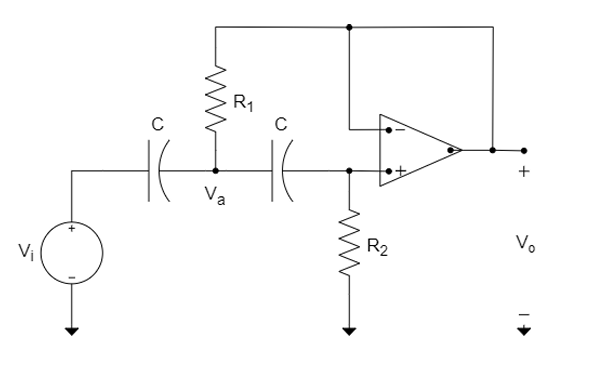
\includegraphics[width=0.5\textwidth]{imgs/filtro_bw.png}
\caption{Diagrama do Primeiro Circuito: Filtro Passa-Altas ButtherWorth 4ª Ordem. (Fonte: \cite{ufpe2023pratica})}
\label{fig:first_circuit_analysis}
\end{figure}

\clearpage

O circuito esperado para o projeto é um filtro Sallen-Key de 4ª ordem.

\begin{figure}[H]
\centering
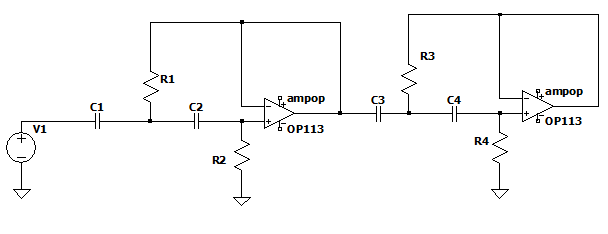
\includegraphics[width=0.8\textwidth]{imgs/sallen-key_de_quarta_ordem.png}
\caption{Diagrama do Circuito Sallen-Key de 4ª Ordem.}
\label{fig:sallen_key_4th_order}
\end{figure}

A função de transferência do circuito é descrita pela seguinte equação:
\begin{equation}
    H_{s} = \frac{C^{4} R_{1} R_{2} R_{3} R_{4} s^{4}}{\left(C^{2} R_{1} R_{2} s^{2} + 2 C R_{1} s + 1\right) \left(C^{2} R_{3} R_{4} s^{2} + 2 C R_{3} s + 1\right)}
    \label{eq:second_transfer_function}
\end{equation}

Sendo assim, possível desenvolver um filtro Butterworth que atende os requisitos do projeto proposto.

\subsection{Projeto do Filtro}

\subsubsection*{Polinômios de Butterworth Normalizados}

Os polinômios de Butterworth podem ser escritos em forma complexa como acima, mas geralmente são escritos com coeficientes reais multiplicando pares de polos que são conjugados complexos, como $s_1$ e $s_n$. Os polinômios são normalizados ajustando $\omega_c = 1$. Os polinômios de Butterworth normalizados têm então a forma geral do produto \cite{kuo1966network}:

\begin{equation}
B_n(s) = \prod_{k=1}^{\frac{n}{2}} \left[s^2 - 2s \cos\left(\frac{2k + n - 1}{2n}\pi\right) + 1\right] \quad \text{n = par}
\end{equation}

\begin{equation}
B_n(s) = (s + 1) \prod_{k=1}^{\frac{n-1}{2}} \left[s^2 - 2s \cos\left(\frac{2k + n - 1}{2n}\pi\right) + 1\right] \quad \text{n = ímpar}
\end{equation} 

O filtro proposto é um filtro passa-altas Butterworth (BW) de 4ª ordem com capacitores de no máximo 100 nF e com a frequência de corte de $f_c = 100$ Hz.

Para um filtro de 4ª ordem, usamos os polinômios de Butterworth normalizados para projetar o filtro. Como tem 2 polos ($k = 1, 2$) e ordem $n = 4$, utilizamos os polinômios de Butterworth normalizados para um filtro projetado de 4ª ordem.

A forma geral dos polinômios de Butterworth normalizados para $n = 4$ é:

\begin{equation}
B_4(s) = \left(s^2 + 0.765367s + 1\right)\left(s^2 + 1.847759s + 1\right)
\end{equation}

A tabela a seguir mostra os fatores dos polinômios de Butterworth de ordem 1 a 10 (com seis casas decimais):

\begin{table}[H]
\scriptsize
\centering
\caption{Factors of Butterworth Polynomials $B_n(s)$}
\begin{tabular}{|c|c|}
\hline
$n$ & Factors of Butterworth Polynomials $B_n(s)$ \\ \hline
1 & $(s + 1)$ \\ \hline
2 & $(s^2 + 1.414214s + 1)$ \\ \hline
3 & $(s + 1)(s^2 + s + 1)$ \\ \hline
4 & $(s^2 + 0.765367s + 1)(s^2 + 1.847759s + 1)$ \\ \hline
5 & $(s + 1)(s^2 + 0.618034s + 1)(s^2 + 1.618034s + 1)$ \\ \hline
6 & $(s^2 + 0.517638s + 1)(s^2 + 1.414214s + 1)(s^2 + 1.931852s + 1)$ \\ \hline
7 & $(s + 1)(s^2 + 0.445042s + 1)(s^2 + 1.246980s + 1)(s^2 + 1.801938s + 1)$ \\ \hline
8 & $(s^2 + 0.390181s + 1)(s^2 + 1.111140s + 1)(s^2 + 1.662939s + 1)(s^2 + 1.961571s + 1)$ \\ \hline
9 & $(s + 1)(s^2 + 0.347296s + 1)(s^2 + s + 1)(s^2 + 1.532089s + 1)(s^2 + 1.879385s + 1)$ \\ \hline
10 & $(s^2 + 0.312869s + 1)(s^2 + 0.907981s + 1)(s^2 + 1.414214s + 1)(s^2 + 1.782013s + 1)(s^2 + 1.975377s + 1)$ \\ \hline
\end{tabular}
\end{table}

Utilizando os polinômios de Butterworth normalizados, as equações $H_1(s)$ e $H_2(s)$ para $k = 1$ e $k = 2$ com $n = 4$ são:

\begin{equation}
H_1(s) = \frac{s^2}{s^2 + 0.765367s + 1}
\end{equation}

\begin{equation}
H_2(s) = \frac{s^2}{s^2 + 1.847759s + 1}
\end{equation}

Deste modo, serão necessários ajustes na escala dos componentes para melhor adequar-se as caracteristicas do filtro.

\subsubsection*{Mudança de Escala}

No projeto e análise de circuitos de filtros passivos e ativos, é conveniente trabalhar com valores de elementos como 1 V, 1 H e 1 F. Depois de fazer cálculos usando esses valores convenientes, o projetista pode transformá-los em valores realistas usando um processo denominado mudança de escala.

Há dois tipos de mudança de escala: amplitude e frequência. Alteramos a escala de amplitude multiplicando a impedância do circuito por um fator de escala $k_a$. Assim, todos os resistores e indutores são multiplicados por $k_a$ e todos os capacitores por $1/k_a$. Se representarmos os valores iniciais dos componentes por R, L e C e os valores dos componentes depois da mudança de escala por $R_r$, $L_r$ e $C_r$, teremos:

\begin{equation}
R_r = k_a R, \quad L_r = k_a L, \quad C_r = \frac{C}{k_a}
\end{equation}

Para mudar a escala de frequência, mudamos os parâmetros do circuito de modo que, na nova frequência, a impedância de cada elemento seja a mesma que era na frequência original. O fator de escala de frequência, $k_f$, é aplicado multiplicando indutores e capacitores por $1/k_f$:

\begin{equation}
R_r = R, \quad L_r = \frac{L}{k_f}, \quad C_r = \frac{C}{k_f}
\end{equation}

A escala de um circuito pode ser mudada em amplitude e frequência simultaneamente:

\begin{equation}
R_r = k_a R, \quad L_r = \frac{k_a}{k_f} L, \quad C_r = \frac{1}{k_a k_f} C
\end{equation}

O uso de capacitores de 100 nF foi escolhido para este projeto devido à sua disponibilidade e ao fato de serem valores práticos para filtros passa-altas em frequências baixas. Com base nos cálculos teóricos, foram determinados os seguintes valores para os resistores do circuito:

\begin{table}[H]
\centering
\caption{Valores Calculados e Comerciais dos Resistores (série E24)}
\begin{tabular}{|c|c|c|}
\hline
\textbf{Resistor} & \textbf{Valor Calculado (k$\Omega$)} & \textbf{Valor Comercial (k$\Omega$)} \\ \hline
R1 & 6,0885577 & 6,2 \\ \hline
R2 & 41,60912 & 42 \\ \hline
R3 & 14,6984577 & 15 \\ \hline
R4 & 17,23388197 & 18 \\ \hline
\end{tabular}
\label{tab:resistor_values}
\end{table}

Com os valores comerciais determinados, podemos proceder para a análise da resposta em frequência do filtro proposto. A próxima seção apresentará o diagrama de Bode do filtro, que é uma ferramenta essencial para visualizar o comportamento do filtro em termos de magnitude e fase.


\subsubsection{Diagrama de Bode do Filtro}
A análise de Bode é essencial para entender o comportamento em frequência do filtro. Os diagramas de Bode de magnitude e fase fornecem uma representação visual da resposta do filtro em frequência e fase ao longo de um intervalo de frequências. Abaixo está o diagrama de Bode para o filtro Sallen-Key de 4ª ordem com os valores de resistores e capacitores discutidos anteriormente.

Para gerar os gráficos, foi utilizada a linguagem Python \cite{python} com as bibliotecas SymPy \cite{sympy} e Matplotlib \cite{matplotlib}.

\begin{figure}[H]
    \centering
    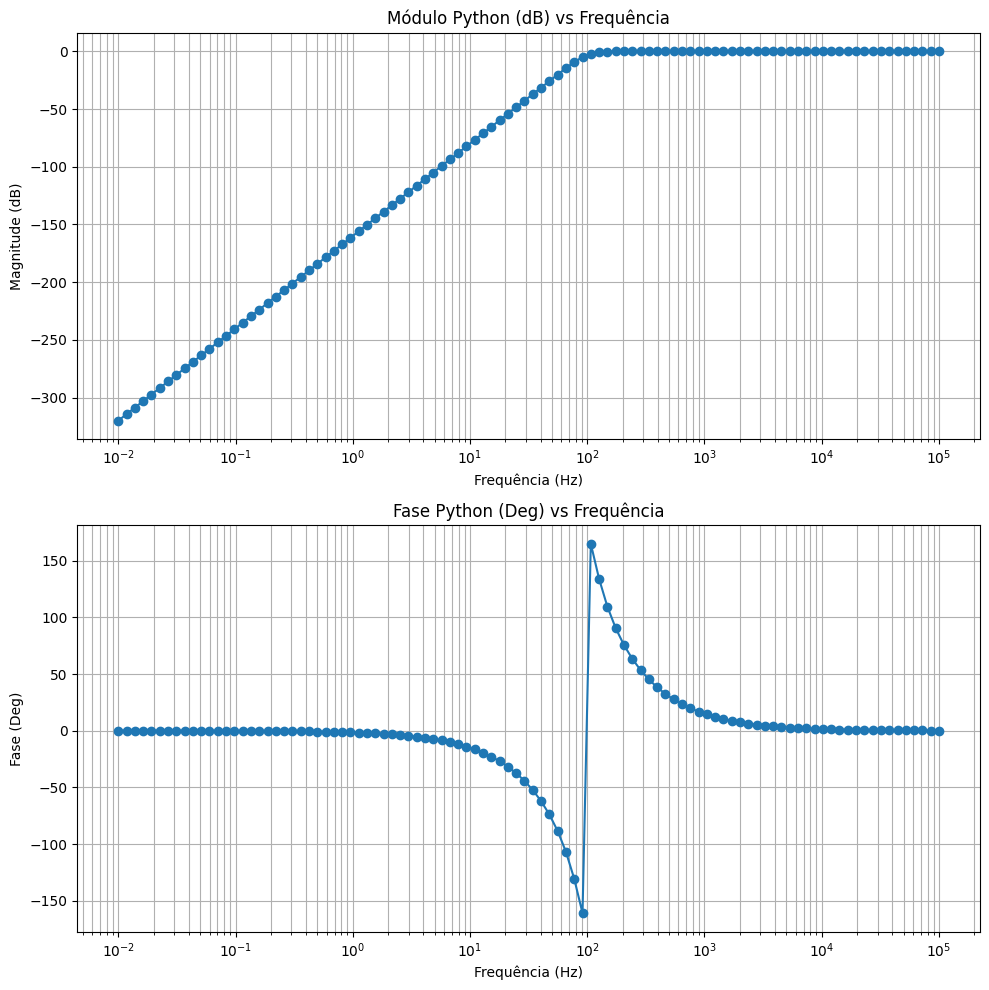
\includegraphics[width=0.85\textwidth]{imgs/output.png}
    \caption{Diagrama de Bode de magnitude e fase do filtro Sallen-Key de 4ª ordem.}
    \label{fig:first_circuit_bode_diagrams}
\end{figure}


Estes diagramas são fundamentais para a análise detalhada do desempenho do filtro em várias frequências. A magnitude mostra como o filtro atenua ou amplifica diferentes frequências, enquanto o gráfico de fase indica a mudança de fase que cada componente de frequência experimenta ao passar pelo filtro.

\subsubsection{Simulação no LTSpice}
Para complementar a análise analítica e os diagramas de Bode, é realizada uma simulação no software LTSpice \cite{ltspice}. A simulação serve para validar o design do filtro e para observar seu comportamento sob condições operacionais simuladas. A seguir, está apresentado o diagrama do circuito montado no LTSpice para o primeiro circuito.

\begin{figure}[H]
    \centering
    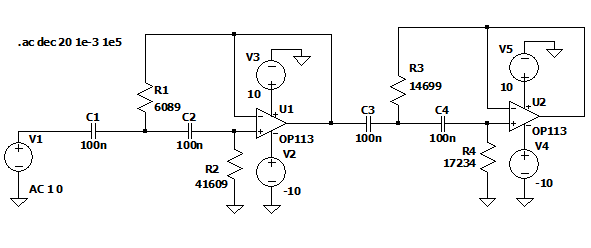
\includegraphics[width=0.8\textwidth]{imgs/circuito_ltspice.png}
    \caption{Diagrama do circuito montado no LTSpice.}
    \label{fig:first_circuit_ltspice_diagram}
\end{figure}

Este diagrama ilustra a configuração do circuito utilizado na simulação, incluindo todos os componentes e conexões necessárias para a análise do filtro passa-altas BW 4ª Ordem . Essa visualização ajuda a garantir que o modelo no LTSpice esteja configurado corretamente conforme o design teórico.

\begin{figure}[H]
    \centering
    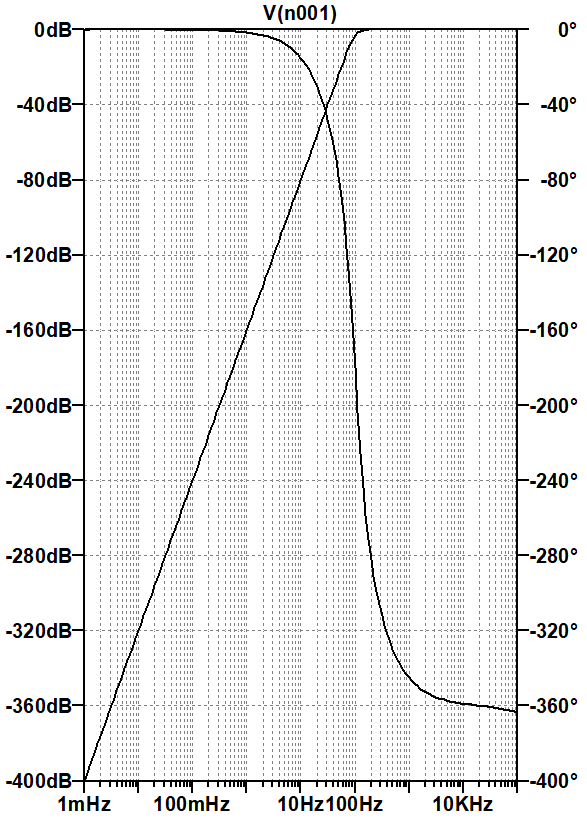
\includegraphics[width=0.8\textwidth,height=0.45\textwidth]{imgs/bode_ltspice.png}
    \caption{Diagrama de Bode do circuito no LTSpice.}
    \label{fig:first_circuit_ltspice_bode}
\end{figure}


O diagrama de Bode gerado pela simulação fornece informações sobre a resposta em frequência do filtro, incluindo a magnitude e a fase. Comparar este diagrama com os resultados analíticos ajuda a identificar qualquer discrepância e a realizar ajustes necessários no design ou na configuração do circuito.



\pagebreak

\chapter{Medições em Laboratório}

Para a segunda parte da prática, o circuito será montado em uma protoboard e serão realizadas medições do sinal de saída, comparando-o com a entrada para determinar a diferença de magnitude e fase da entrada para a saída.

\section{Medição dos Componentes com Multímetro}

Utilizando um multímetro, os valores dos resistores e capacitores do circuito serão medidos e registrados. A tabela abaixo compara os valores esperados com os valores mensurados:

\begin{table}[H]
    \small
    \scriptsize
    \centering
    \begin{tabular}{|c|c|c|}
        \hline
        Componente & Valor Esperado & Valor Mensurado \\
        \hline
        Capacitor (C) & 100 nF & 101 nF \\
        Resistor (R1) & 6,088 k\(\Omega\) & 5,50 k\(\Omega\) \\
        Resistor (R2) & 41,609 k\(\Omega\) & 37,9 k\(\Omega\) \\
        Resistor (R3) & 14,698 k\(\Omega\) & 14,7 k\(\Omega\) \\
        Resistor (R4) & 17,234 k\(\Omega\) & 17,3 k\(\Omega\) \\
        \hline
    \end{tabular}
    \caption{Comparação dos valores esperados e mensurados dos componentes com multímetro \cite{keysight-u1250}}
    \label{tab:component_values}
\end{table}

Neste estágio, as medições reais ainda serão realizadas e os valores mensurados preenchidos posteriormente, permitindo a validação dos cálculos teóricos com os dados práticos.

\section{Montagem do Circuito na Protoboard}

O circuito será montado na protoboard. Após a montagem, a fonte de tensão será conectada para alimentar o circuito. A figura abaixo mostra o circuito montado na protoboard.

\begin{figure}[H]
    \centering
    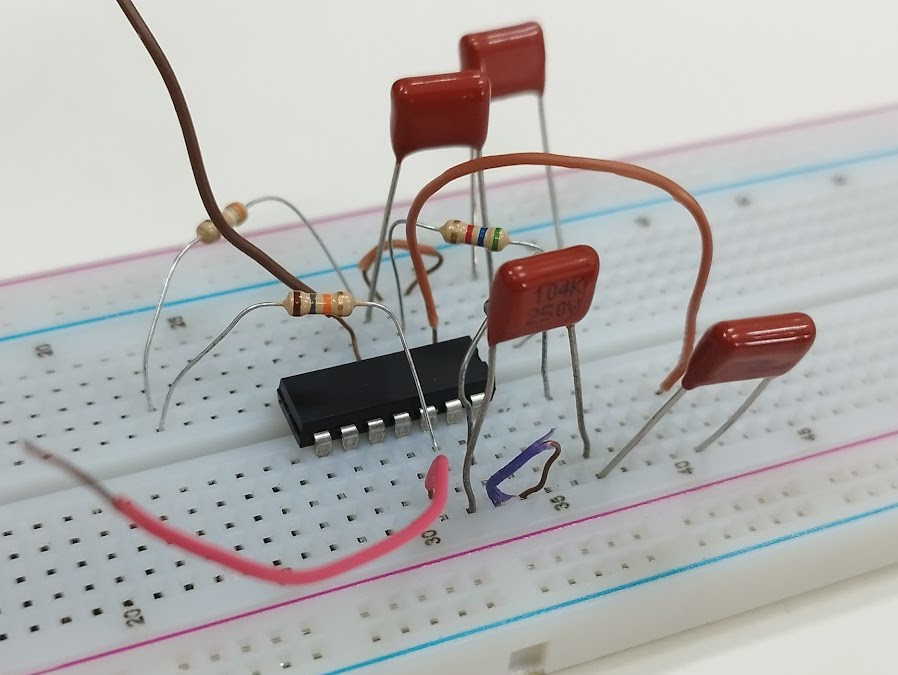
\includegraphics[width=0.6\textwidth]{imgs/circuito_protoboard.jpg}
    \caption{Montagem do circuito na protoboard.}
    \label{fig:circuito_protoboard}
\end{figure}

\pagebreak

\subsection{Configuração do Osciloscópio}

O gerador de sinal do osciloscópio será conectado na entrada \( v_i(t) \) do circuito. O gerador será configurado para gerar uma onda senoidal de amplitude de 5 V pico a pico. A frequência será ajustada conforme os passos abaixo. Com a entrada do circuito no canal 1 e a saída no canal 2 do osciloscópio, ligue a fonte de tensão e o gerador de sinais. A figura abaixo mostra as amplitudes das tensões de entrada e de saída para uma frequência de 1 kHz. Esses valores serão utilizados para determinar o ganho do filtro para frequências altas.

\begin{figure}[H]
    \centering
    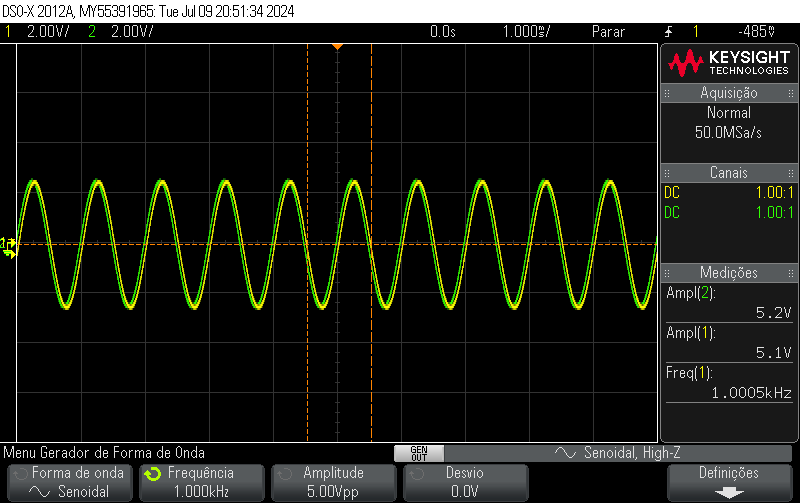
\includegraphics[width=0.8\textwidth]{imgs/scope_7.png}
    \caption{Curva de saída no osciloscópio para uma frequência de 1 kHz.}
    \label{fig:high_frequency_output}
\end{figure}


\subsection{Cálculo da Tensão Máxima}

Com base na máxima tensão de saída observada de 5.2V, o valor de \( H_{\text{max}} \) é calculado da seguinte forma:

\begin{equation}
H_{\text{max}} = \frac{1}{\sqrt{2}} \times 5.2 \approx 3.6769 \text{V}
\end{equation}

Este valor será utilizado para análises adicionais.


\subsection{Frequência de Corte Observada}
A frequência de corte observada, onde a amplitude de saída cai para 70.7\% da amplitude máxima observada, foi determinada como 100,34 Hz (ver Figura \ref{fig:first_oscilloscope_cutoff_frequency}). Esta informação é essencial para validar a performance do filtro em atenuar frequências acima deste ponto.


\begin{figure}[H]
    \centering
    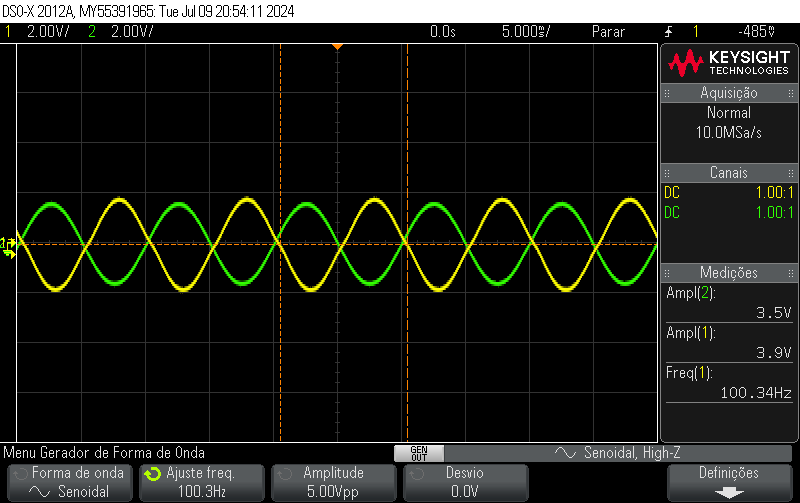
\includegraphics[width=0.75\textwidth]{imgs/scope_9.png}
    \caption{Curva de saída no osciloscópio mostrando a frequência de corte.}
    \label{fig:first_oscilloscope_cutoff_frequency}
\end{figure}

Este procedimento assegura uma compreensão detalhada da característica passa-baixa do filtro e da influência da frequência sobre a amplitude do sinal.

\subsection{Medição de Amplitudes em Frequências Variadas}

A amplitude de saída será medida para diferentes frequências para avaliar a frequência de corte do filtro. As amplitudes de entrada e saída para cada frequência testada serão registradas na seguinte tabela:

\begin{table}[H]  
    \scriptsize
    \centering
    \begin{tabular}{|c|c|c|}
        \hline
        Frequência (Hz) & Amplitude de Entrada (Vi) (V) & Amplitude de Saída (Vo) (V) \\
        \hline
        15 & 5.1 & 0 \\
        50 & 5.1 & 0.34 \\
        75 & 5.1 & 1.33 \\
        100 & 5.1 & 3.26 \\
        125 & 5.1 & 4.7 \\
        150 & 5.1 & 5.09 \\
        200 & 5.1 & 5.21 \\
        \hline
    \end{tabular}
    \caption{Amplitudes de entrada e saída para diferentes frequências.}
    \label{tab:frequency_response}
\end{table}

Este procedimento assegura uma compreensão detalhada da característica passa-altas do filtro e da influência da frequência sobre a amplitude do sinal.


\pagebreak
\chapter{Resultados}

Os resultados obtidos a partir das medições laboratoriais, teóricas e simulações revelam comportamentos característicos do filtro passa-altas Sallen-Key de 4ª ordem. A análise focou na avaliação da frequência de corte, na máxima tensão de saída e na forma como esses elementos se alinham com as previsões teóricas das funções de transferência.

\section{Características Observadas no Circuito}

O circuito exibiu a propriedade fundamental de um filtro passa-altas, que é a manutenção da máxima tensão de saída em frequências altas. Como foi teoricamente previsto e confirmado pelas simulações e medições em laboratório, a amplitude da saída aumenta conforme a frequência de entrada excede a frequência de corte. Esta característica foi visualmente confirmada pelos gráficos de Bode (ver Figura \ref{fig:first_circuit_bode_diagrams}), que mostraram uma resposta de ganho crescente próximo à frequência de corte do filtro.

\subsection{Análise da Função de Transferência}

A função de transferência do circuito, detalhada na equação \ref{eq:second_transfer_function}, fundamenta o comportamento observado. A frequência de corte do filtro foi calculada e medida, mostrando uma boa concordância entre os valores teóricos e os valores obtidos experimentalmente. As medições foram realizadas conforme descrito na seção de configuração do osciloscópio e mostraram resultados consistentes com o esperado.

\subsection{Comparação das Frequências de Corte}

Interessante observar que, apesar de variações mínimas nos valores dos componentes utilizados, a frequência de corte observada foi bastante precisa e consistente com as previsões teóricas. A escolha dos valores dos resistores e capacitores foi crucial para garantir que o filtro operasse conforme o esperado, destacando a importância de selecionar corretamente os componentes durante o design.

\section{Síntese dos Resultados}

Os dados consolidados oferecem uma visão ampla da eficácia do design do filtro e da adequação das técnicas de simulação e medição. As análises teóricas se alinham bem com as observações práticas, o que confirma a validade dos modelos teóricos utilizados e proporciona uma base sólida para futuras iterações de design e otimização.



\chapter{Conclusão}

Esta atividade validou a eficácia do filtro passa-altas Sallen-Key de 4ª ordem, confirmando a consistência entre teoria, simulações e resultados experimentais. O circuito investigado aderiu ao princípio fundamental de maximizar a tensão de saída em frequências altas e atenuar as baixas.

As análises realizadas demonstram que simulações e medições são métodos eficazes para validar a performance do filtro. Além disso, recomenda-se a realização de pesquisas adicionais para explorar o impacto de variáveis externas, como a temperatura, no desempenho do filtro a longo prazo.

Portanto, este estudo enfatiza a importância de métodos de simulação e medição precisos para o desenvolvimento e validação de componentes eletrônicos, servindo como um guia prático para futuras inovações na engenharia eletrônica.




\clearpage
\bibliography{bibliografia}



\end{document}

% ----------------------------------------------------------
% ELEMENTOS PÓS-TEXTUAIS
% ----------------------------------------------------------
\postextual

% ----------------------------------------------------------
% Referências bibliográficas
% ----------------------------------------------------------
\bibliography{bibliografia}

% ----------------------------------------------------------
% Glossário
% ----------------------------------------------------------
%
% Consulte o manual da classe abntex2 para orientações sobre o glossário.
%
%\glossary



\end{document}
